% "Станет проще"

\documentclass[a4paper,12pt]{article} % тип документа

% report, book

% Рисунки
\usepackage{graphicx}
\usepackage{wrapfig}
\usepackage{hyperref}
\usepackage[rgb]{xcolor}
\pagestyle{plain}



%  Русский язык

\usepackage[T2A]{fontenc}			% кодировка
\usepackage[utf8]{inputenc}			% кодировка исходного текста
\usepackage[english,russian]{babel}	% локализация и переносы


% Математика
\usepackage{amsmath,amsfonts,amssymb,amsthm,mathtools} 


\usepackage{wasysym}

%Заговолок
\author{Сафиуллин Роберт	}
\title{Лабораторная работа 3.4.4\\ Петля гестерезиса
(статистический метод)}





\begin{document} % начало документа

\maketitle


\newpage
\section{Цель работы:}
исследование кривых намагничивания ферромагнетиков с помощью баллистического гальванометра.
\\
\section{В работе используются:}
генератор тока, блок питания, тороид, соленоид, баллистический гальванометр с осветителем и шкалой, амперметры, магазин сопротивлений, ЛАТР, разделительный трансформатор.

 
\section{Экспериментальная установка:}
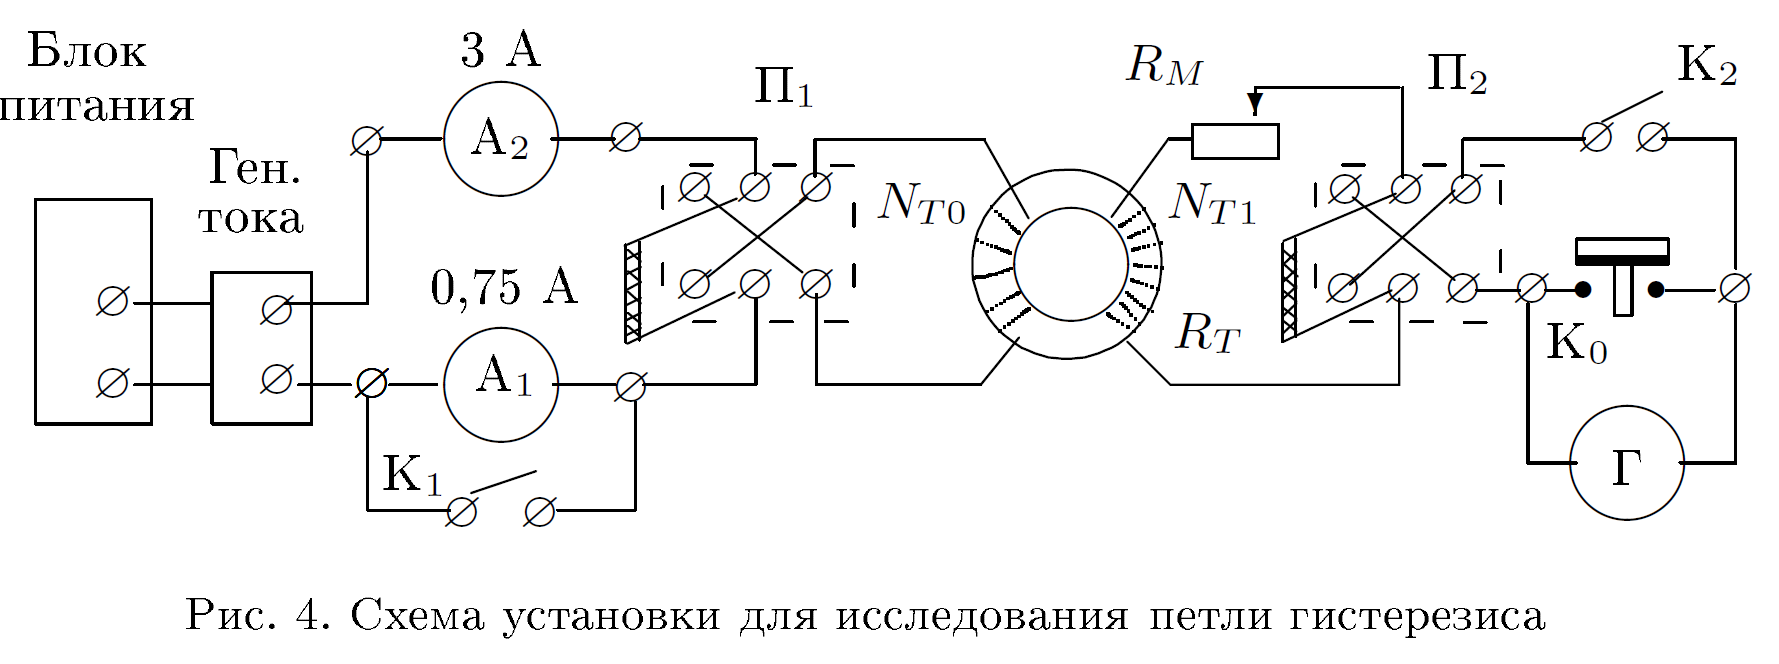
\includegraphics[scale=0.35]{ust}\\
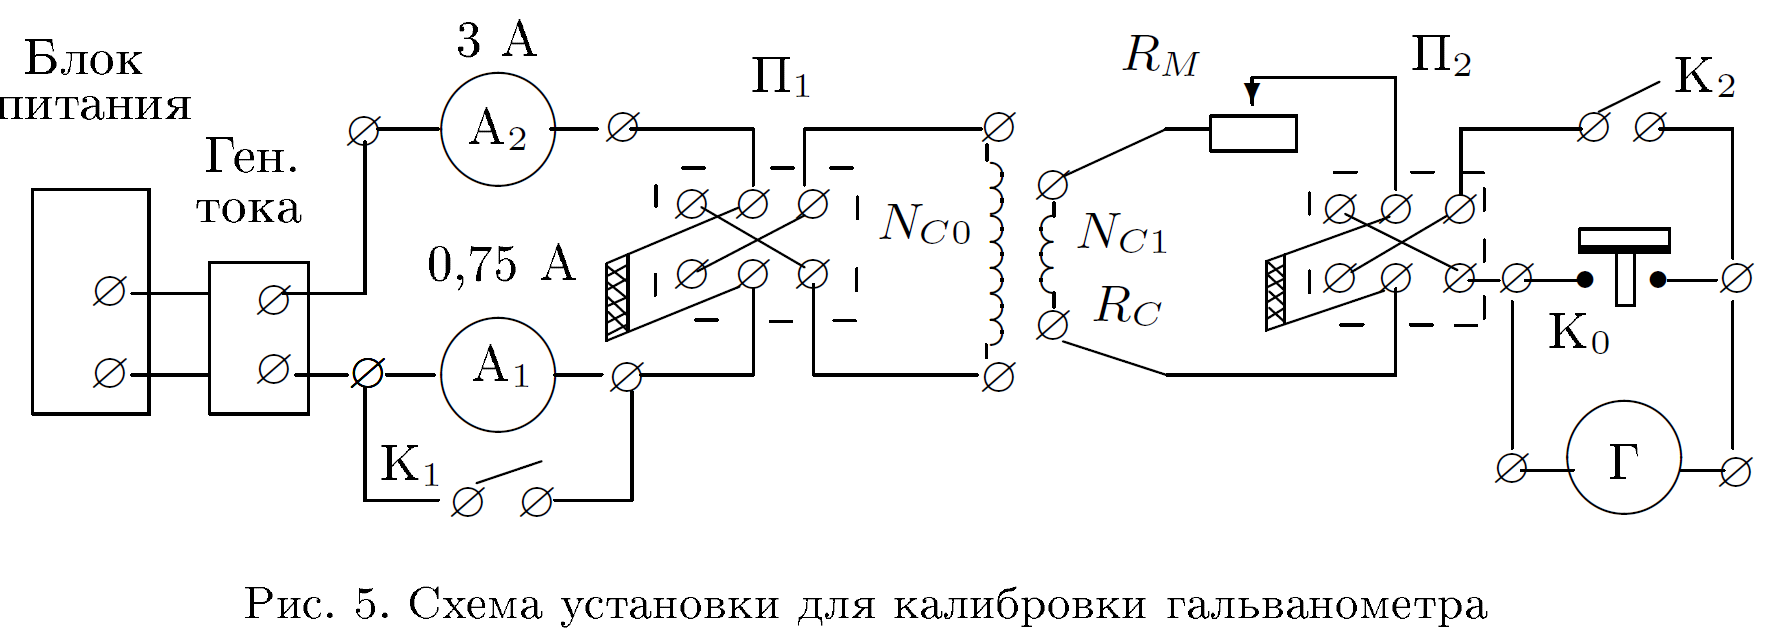
\includegraphics[scale=0.35]{ust1}\\
$d_c=7 cm \quad
R_0=50 \Omega \quad
R_c=60 \Omega    \quad
           R_M=100 \Omega\quad
              l_c=80 cm \\
N_{C0}=825\quad
N_{C1}=435\quad
N_{T1}=300 \quad
N_{T0}=1750$


\section{Ход работы}

1) Сoбрали схему 4 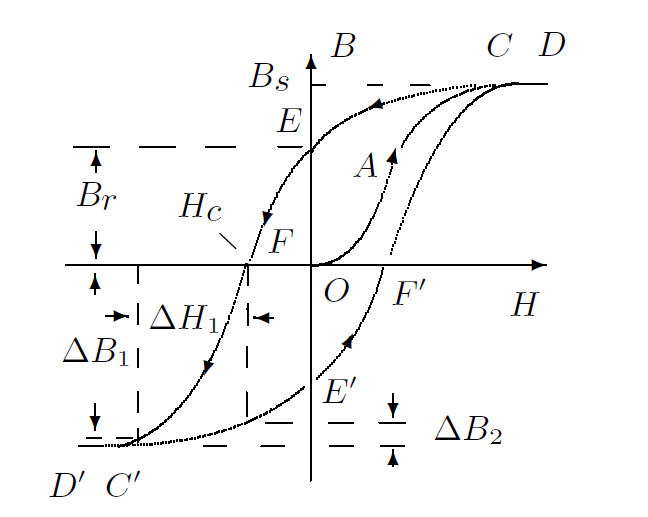
\includegraphics[scale=0.5]{ge} \\
2) Установили сопротивление 80 $\Omega$ и прошли по всей петле.\\
3) Убедившись, что зайчик нигде не выходит за шкалу, снимем\\ показания: \\
\begin{tabular}{|c|c|c|c|}
\hline
\multicolumn{4}{|c|}{Участок CE} \\ 
\hline
I, mA & $\Delta$x,cm & H, A/m & $\Delta B$, Тл \\ 
\hline 
1470 & 0 & 8192 & 0 \\ 
\hline 
530 & 12 & 2954	 &0.22 \\ 
\hline 
244 & 12 & 1360 & 0.22\\ 
\hline 
147 & 8.6 & 819 & 0.16		\\ 
\hline 
96 & 6.6 & 535 & 0.12 \\ 
\hline 
65 & 5.1 & 362 & 0.092 \\ 
\hline 
50 & 3 & 279 & 0.05\\ 
\hline 
40 & 2 & 223 & 0.036\\ 
\hline 
34 & 1.2 & 189 & 0.022 \\ 
\hline 
31 & 0,7 & 173 & 0.012 \\ 
\hline 
27 & 1 & 150 & 0.018 \\ 
\hline 
23 & 0.9 & 128 & 0.016\\ 
\hline 
0.6 & 7.2 & 3.34 & 0.13\\ 
\hline 
0,00032 & 0.1 & 0.002 & 0.0018\\ 
\hline 
\end{tabular} 
\begin{tabular}{|c|c|c|c|}
\hline 
\multicolumn{4}{|c|}{Участок EF'C'} \\ 
\hline
I, mA & $\Delta$x,cm & H, A/m & $\Delta B$, Тл \\
\hline 
0.00032 & 0 & 0.002 &0 \\ 
\hline 
0.6 & 0.1& 3.34 &0.0018 \\ 
\hline 
23 & 12& 128 &0.22 \\ 
\hline 
27 & 2.9 & 150 &0.053 \\ 
\hline 
31 &  4.1& 173 & 0.07\\ 
\hline 
34 & 4.6& 189 & 0.083 \\ 
\hline 
40 & 13.6& 223 & 0.25 \\ 
\hline 
50 & 23& 279 & 0.42\\ 
\hline 
65 & 22& 362& 0.4 \\ 
\hline 
96 & 21.5& 535 & 0.39 \\ 
\hline 
147 & 16.6 & 819 & 0.3\\ 
\hline 
244 & 15.6& 1360 & 0.28 \\ 
\hline 
540 & 19.2& 2954 & 0.35 \\ 
\hline 
1470 & 15.4 & 8192 & 0.28\\ 
\hline 

\end{tabular} 
\\
\begin{tabular}{|c|c|c|c|}
\hline 
\multicolumn{4}{|c|}{Участок C'E'} \\ 
\hline
I, mA & $\Delta$x,cm & H, A/m & $\Delta B$, Тл \\
\hline 
1470 & 0 &  8192     &  0  \\ 
\hline 
530 & 12.2 &    2954   &0.22 \\ 
\hline 
244 & 12.4 &     1360  & 0.23 \\ 
\hline 
147 & 9&    819   & 0.16 \\ 
\hline 
96 & 6.7&    535   & 0.12 \\ 
\hline 
65 & 5.1&     362  &  0.09\\ 
\hline 
50 & 3 &279       & 0.05\\ 
\hline 
40 & 2 &   223    & 0.036 \\ 
\hline 
34 & 1.2&  189     & 0.022 \\ 
\hline 
31 & 0.6 &    173   & 0.011 \\ 
\hline 
27 & 1&    150   &0.018  \\ 
\hline 
23 & 0.9&  128      & 0.016 \\ 
\hline 
0.6 & 7.4&    3.34   & 0.13 \\ 
\hline 
0,00032 & 0.1&    0.002   & 0.002 \\ 
\hline 
\end{tabular} 
\begin{tabular}{|c|c|c|c|}
\hline 
\multicolumn{4}{|c|}{Участок OAC} \\ 
\hline
I, mA & $\Delta$x,cm & H, A/m & $\Delta B$, Тл \\

\hline 
0.00032 & 0&0.002       & 0  \\ 
\hline 
0.6 & 0.1 &   3.34    & 0.002 \\ 
\hline 
23 & 12.4 &    128   & 0.23 \\ 
\hline 
27 & 2.9 &  150     & 0.05 \\ 
\hline 
31 &  4.1&     173  & 0.074 \\ 
\hline 
34 & 4.6 &     189  & 0.08\\ 
\hline 
40 & 14&    223   & 0.25 \\ 
\hline 
50 & 25 &   279    & 0.45\\ 
\hline 
65 & 23&   362    &  0.42\\ 
\hline 
96 & 23&535       &  0.42\\ 
\hline 
147 & 17.7&819       & 0.32 \\ 
\hline 
244 & 16.2&   1360    & 0.29 \\ 
\hline 
540 & 20.8&    2954   & 0.38 \\ 
\hline 
1470 & 16.1&     8192  & 0.3 \\ 
\hline 

\end{tabular} 


4) Для калибровки гальванометра собрали схему 5. Уменьшили на магазине сопротивлений значение $R_M$ на величину $R_C$: $R_M$'= 20 $\Omega$. Установили тумблер генератора тока на максимум и , замкнув ключ $\Pi_1$ $, запишем значение I_{max}=1.87 A$. Разомкнули ключ  $\Pi_1$ и измерили отклонение $\Delta x_1$=9.2 cm при $\Delta I_1=I_{max}$. \\
5) Снимем начальную кривую намагничивания с помощью схемы 4. Перед этим размагнитим образец при помощи ЛАТРа. \\
\begin{center}

\begin{tabular}{|c|c|c|c|}
\hline 
\multicolumn{4}{|c|}{Участок E'F'C} \\ 
\hline
I, mA & $\Delta$x,cm & H, A/m & $\Delta B$, Тл \\
\hline 
0.56 & 0 &3.12 & 0\\ 
\hline 
24 & 5.5&133.8 & 0.102 \\ 
\hline 
28 & 2.2& 156& 0.04 \\ 
\hline 
31.5 & 3.1&175 &0.06 \\ 
\hline 
34.1 & 3& 190& 0.56\\ 
\hline 
50 & 9.1 &279 &0.17\\ 
\hline 
65.2 & 11.3& 363& 0.21 \\ 
\hline 
96.4 & 15.1& 537& 0.28\\ 
\hline 
147 & 14.2&819 &  0.263\\ 
\hline 
244 & 14.9&1360 &  0.276\\ 
\hline 
540  & 18.9&3010 &0.35 \\ 
\hline 
1470  & 15.4& 8193& 0.286\\ 
\hline 
40.1 & 6.5& 223.5 & 0.12\\ 
\hline 
\end{tabular} 

\end{center}

 6) Обработаем результаты, используя формулы: \\
$H = I\frac{N_{T0}}{\pi D_{tor}}$\\
$\Delta B [T]$ = $\mu_0$ $(\frac{d_c}{d_T})^2  \frac{R_{tor}}{R_{sol}}  \frac{N_{C0}}{N_{T1}} \frac{N_{C1}}{l_C} \Delta I_1 \frac{\Delta x}{\Delta x_1}  , d_T=1 cm, D_{tor}=10 cm.$ \\
Результаты занесем в первые таблицы.\\
7) Построим петлю гестерезиса: \\
\begin{flushleft}


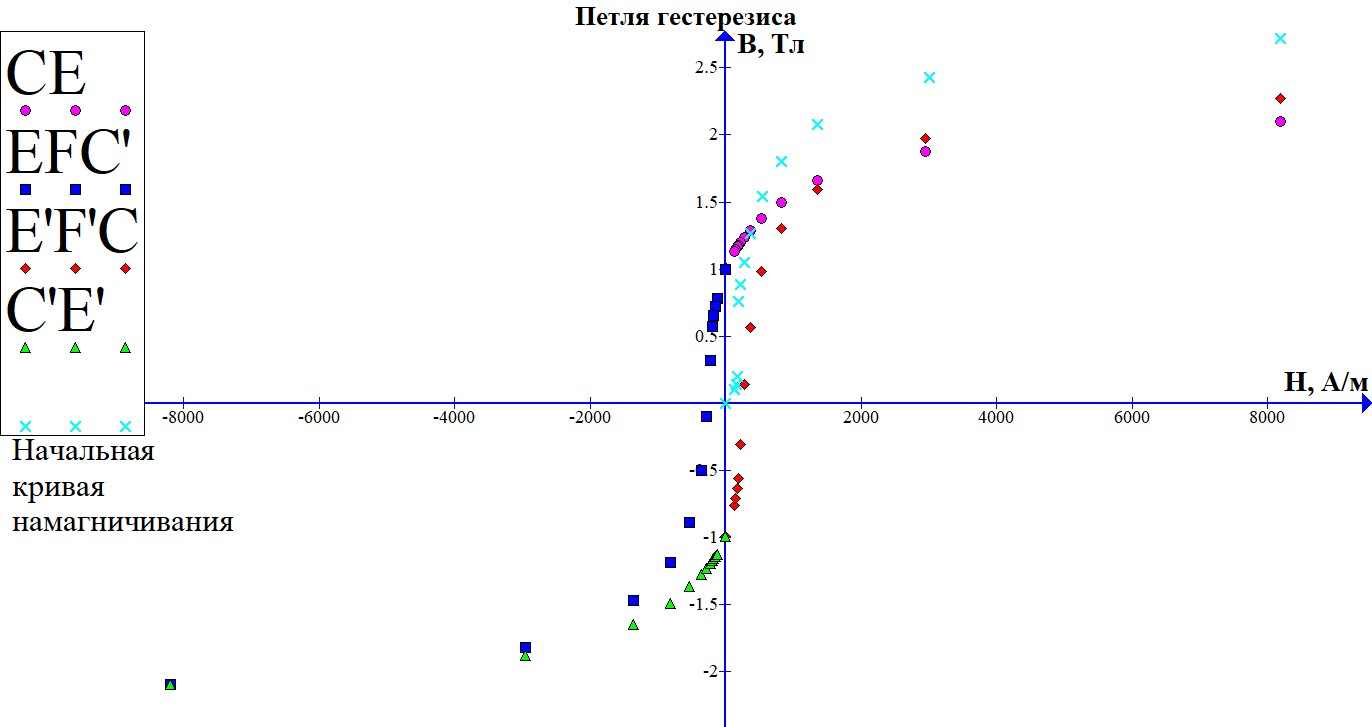
\includegraphics[scale=0.36]{3441}


\end{flushleft}




Отсюда $H_c\approx580 A/m, B_s=2.23$ Тл\\
\begin{center}

\begin{tabular}{|c|c|c|}
\hline 
• & Эксперим. & Табличное \\ 
\hline 
$H_c,  \frac{A}{m}$ & 580 & 80 \\ 
\hline 
$B_s, T$ & 2.23 & 2.15 \\ 
\hline 
$\mu_{dif}$ & 12200 & 5000 \\ 
\hline 
\end{tabular} 
\end{center}

































\end{document} % конец документа
